\chapter{Realization}\label{ch:B}

\section{Functional requirements}
 
Taking into account the results of analyses, interviews and surveys, we have made the main functionality. The main idea of our project make a single platform for charitable activities. And the main functionality and backlogs will be:
\begin{itemize}
    \item \textbf{Provide only reliable hands that open and manage feeds} 
    
        To solve the problem of distrust of charitable collections and foundations, we have come up with a functional in which each user has the opportunity to open his own fund. But in order to open the find, the user must have the appropriate documents and evidence of the presence of only official funds in the application. Fund managers have full access to fund management and fees
    
    \item \textbf{Make a reliable donation functionality}
    
        Each user has the opportunity to send a request to open a collection. For an open collection, you need to create an application that requires supporting documents and collection data, and therefore the user can send these applications to official funds. Follow-up actions the heads of charitable foundations, after reviewing the list of applications, can contact the user and open the collection. This way we can solve the problem of distrust and fraud
        
    \item \textbf{Make functionality for full reporting of fees}
    
        In applications, each charity collection has statistics and reports. For example, the application will display how much interest has already been collected, how much in total the amount has been collected, and how much amount is left. When the amount has reached the limit, the collection is automatically closed. Since everything is automated, no human actions are required here. This way we can solve the problem with fundraise reports.
        
    \item \textbf{Make functionality to provide news about food and clothing or other donations} 
    
        In the application, you can see active collection points for various purposes (clothing, food, etc.). The map will display information on the opening hours of the points and additional information
        
        
        
        
\end{itemize}

\section{User Interface}

A user interface is a way of interacting between a user and an interface. Designing the
application interface for mobile devices, we took into account the features and requirements of the operating system. Therefore, in order to create a user-friendly interface in which the user can easily understand the application and navigate through it effectively, we took into account the Human Interface Guidelines for IOS, and also used GUI elements such as: \cite{design}

\begin{itemize}
    \item Button is an element that an action takes place when clicked.
    \item Content — text, images, that is, the content of the interface
    \item Text field — a field for entering text values
    \item Menu - contains a list of options, and allows you to choose one of the options
    \item TabBar is a tab bar at the bottom of the screen that allows you to quickly switch between sections of the application.
    \item Progress Bar — indicator of the degree of completion of an action
    \item Onboarding is a learning functionality in the application that appears at the first launch to familiarize the user with the application
    \item Icons is a small clickable image, a part of the graphical interface that facilitates the visual search for the function associated with it
\end{itemize}

\subsection{User Personas}

    Before starting to create a design, we conducted a thorough research. This is done in order to understand the user and his pain points in order to satisfy them. Based on the research data, we have created user persona, user flow and information architecture. The user persona describes the person who will interact with the product. Most often, this
    person is given a fictitious name, but the rest of the information is generalized information based on the result of research aimed at collecting information about users using various qualitative and quantitative methods.  We have compiled 4 different user portraits.
    
    % user personas images
    \begin{center}
        \begin{tabular}{ c  c }
            \begin{minipage}{0.2\textwidth}
                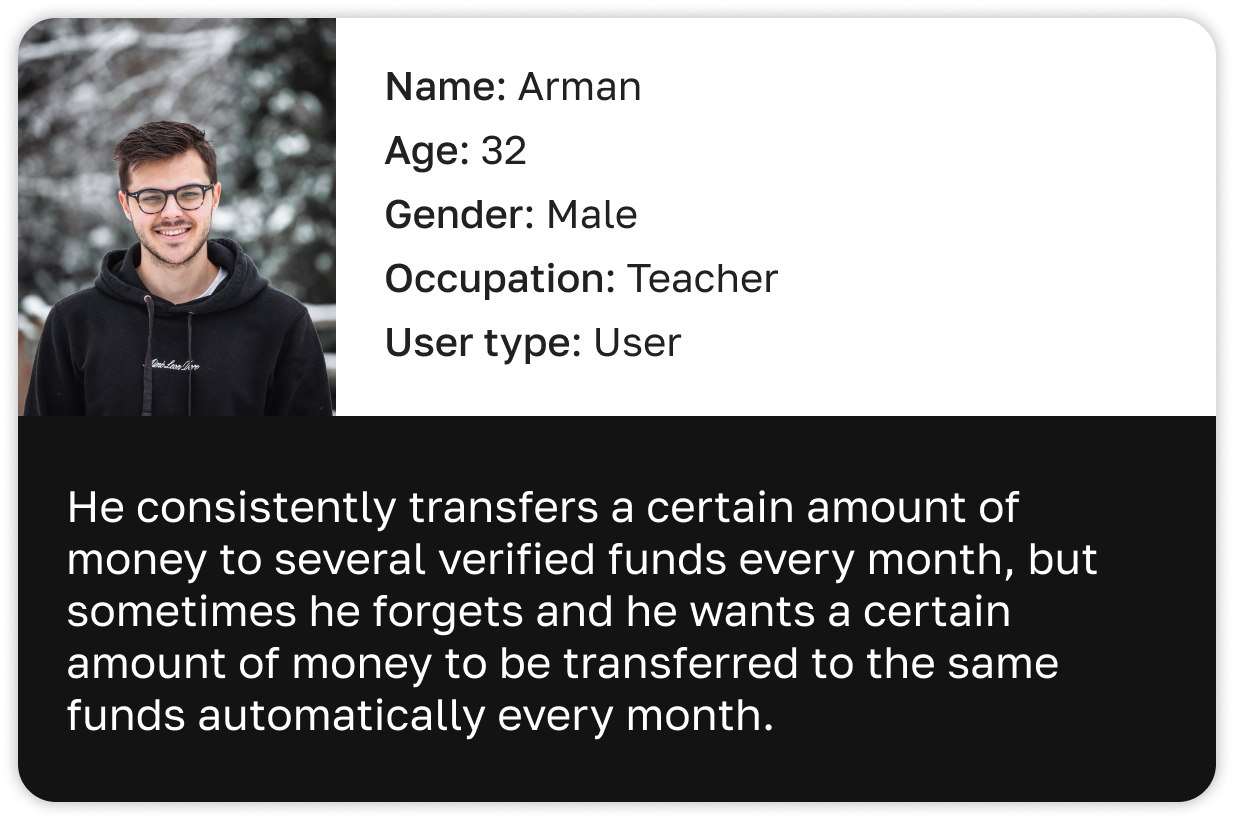
\includegraphics[scale=0.2]{figures/userPersonas/User-persona 01.jpg}
            \end{minipage} \hspace*{0.5cm} & \begin{minipage}{0.2\textwidth}
                    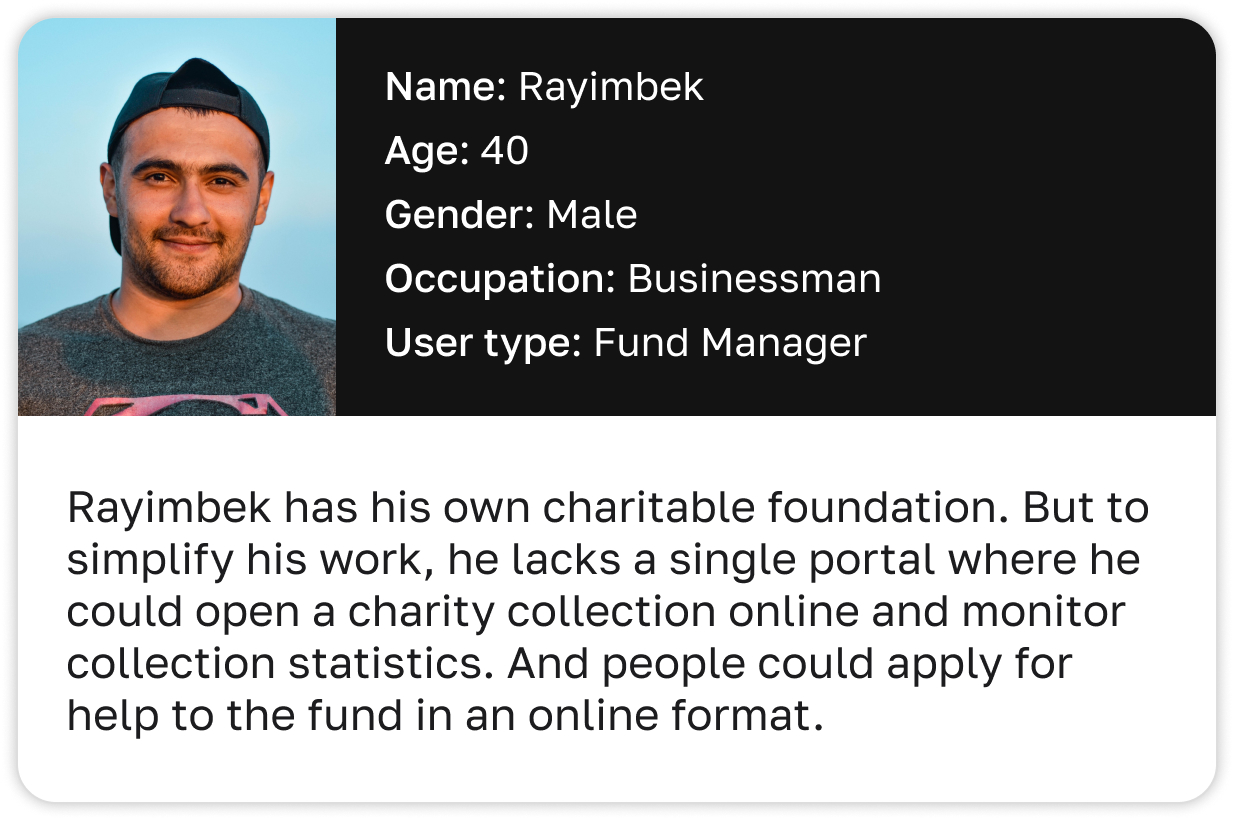
\includegraphics[scale=0.2]{figures/userPersonas/User-persona 02.jpg}
                \end{minipage}   \\
            \begin{minipage}{0.2\textwidth}
                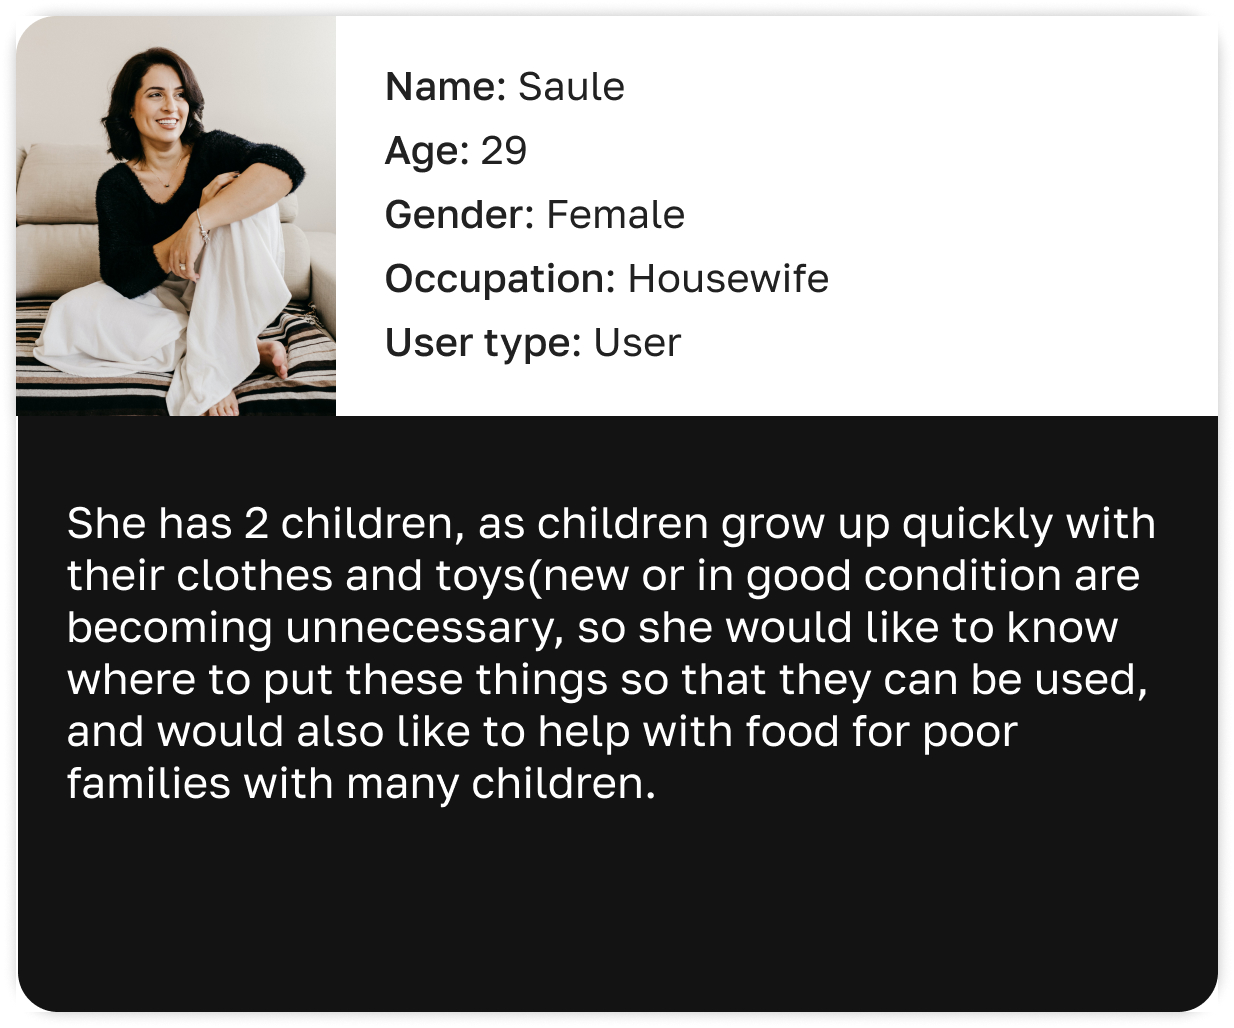
\includegraphics[scale=0.2]{figures/userPersonas/User-persona 03.jpg}
            \end{minipage} \hspace*{0.5cm} & \begin{minipage}{0.2\textwidth}
                    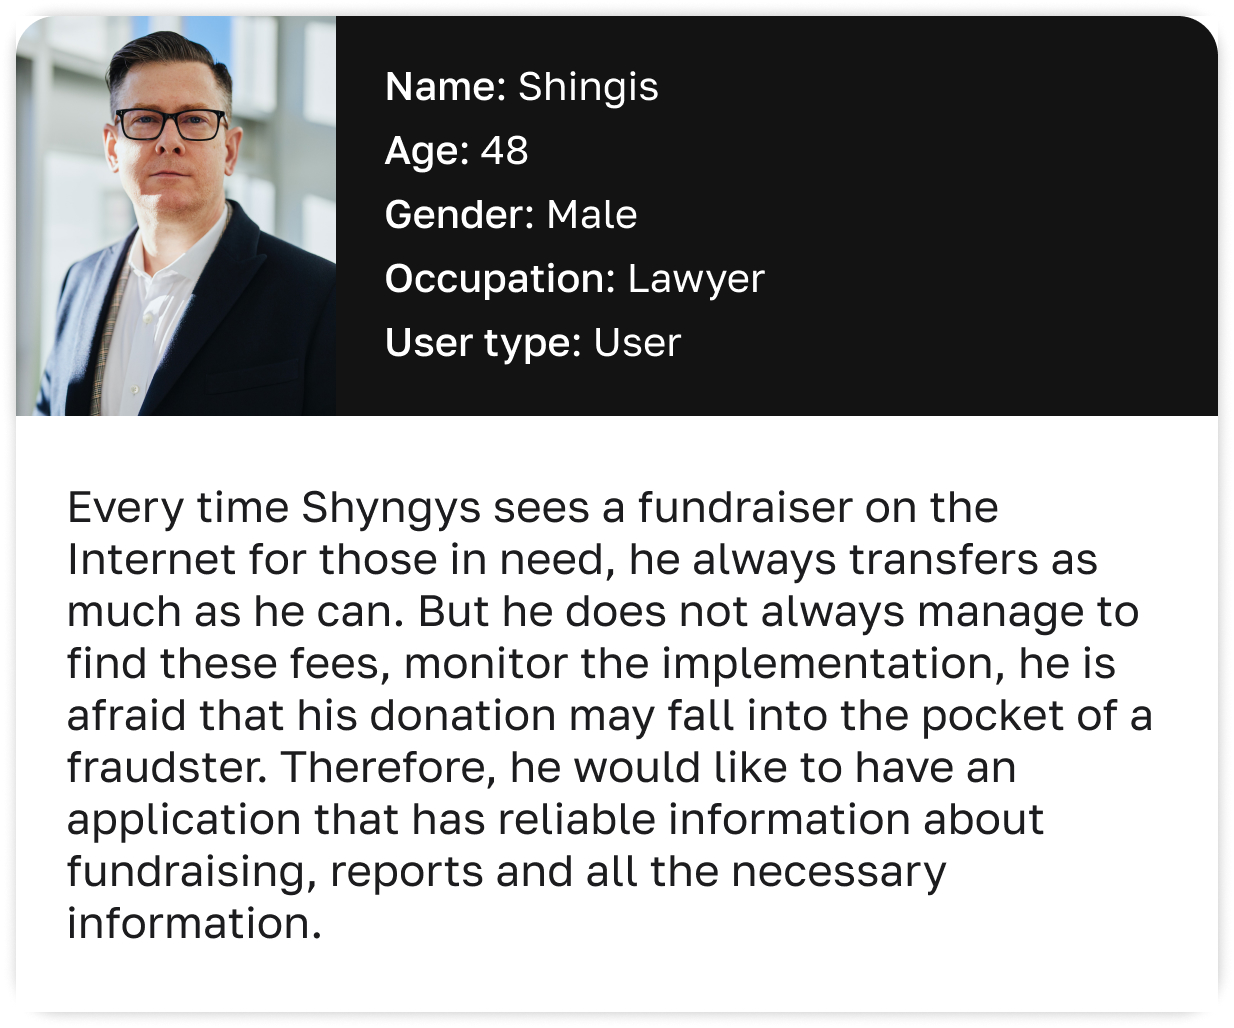
\includegraphics[scale=0.2]{figures/userPersonas/User-persona 04.jpg}
                \end{minipage}  \\
        \end{tabular}
    \end{center}
    
\subsection{User Stories}
    
User stories step-by-step describes the user's goal, which he wants to achieve with the
application, and its ultimate benefit. As a result, we received a list of requirements that allowed us to determine the functionality of the future application and make it as user-friendly as possible.

Our user stories were:

As a user, I want to see a list of funds

As a user, I want to see every functionality in one page

As a user, I want to see the location of delivery points on the map

As a user, I want to see a list of collection of funds

As a user, I want to see the required and collected collection amount

As a user, I want to make a donation to a certain fundraiser...

\subsection{User Flow}

We needed User flow in order to visually see the sequence of user actions that he performs to achieve his goal.

\begin{figure}[h]
    \centering
    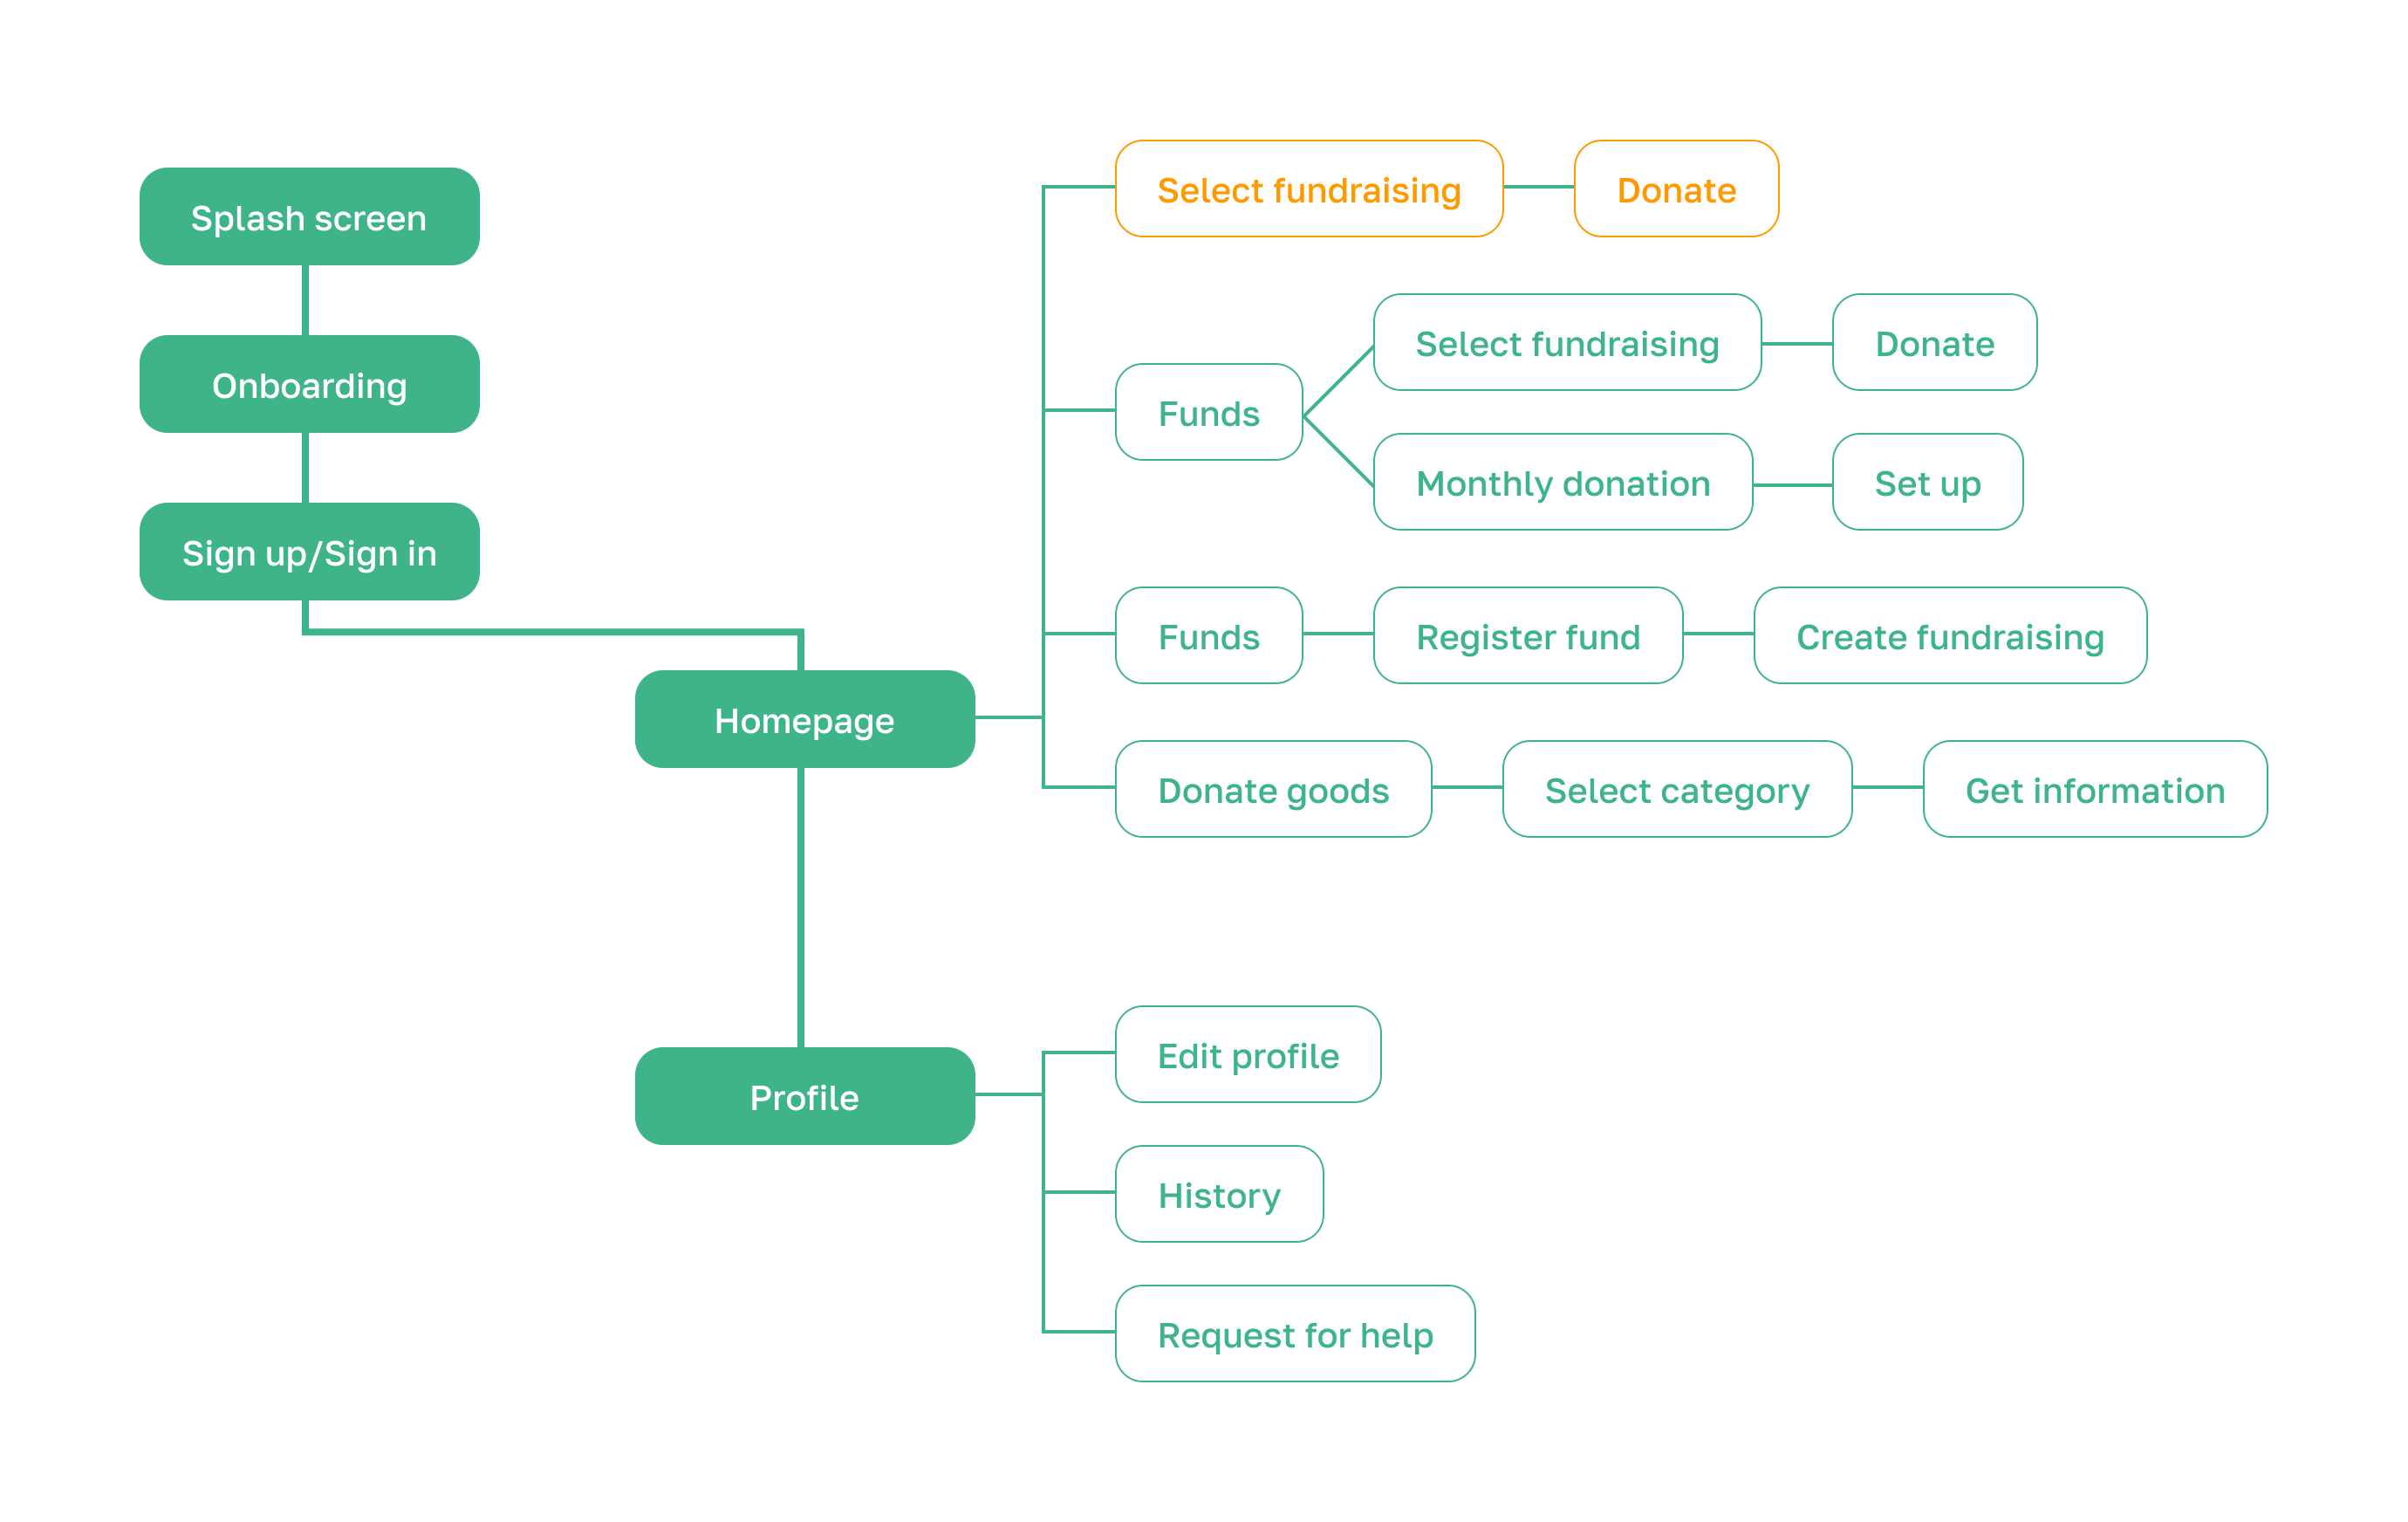
\includegraphics[width=10cm]{figures/userInterface/user flow.jpg}
    \caption{User Flow}
    \label{fig:userFlow}
\end{figure}
% userFlow image

\subsection{Information Architecture}

After UX research, we started creating an information architecture. To do this, we have created a site map, a mind map. We used the \textbf{sitemap} to hierarchically display the relationship between pages.

% sitemap image
\begin{figure}[h]
    \centering
    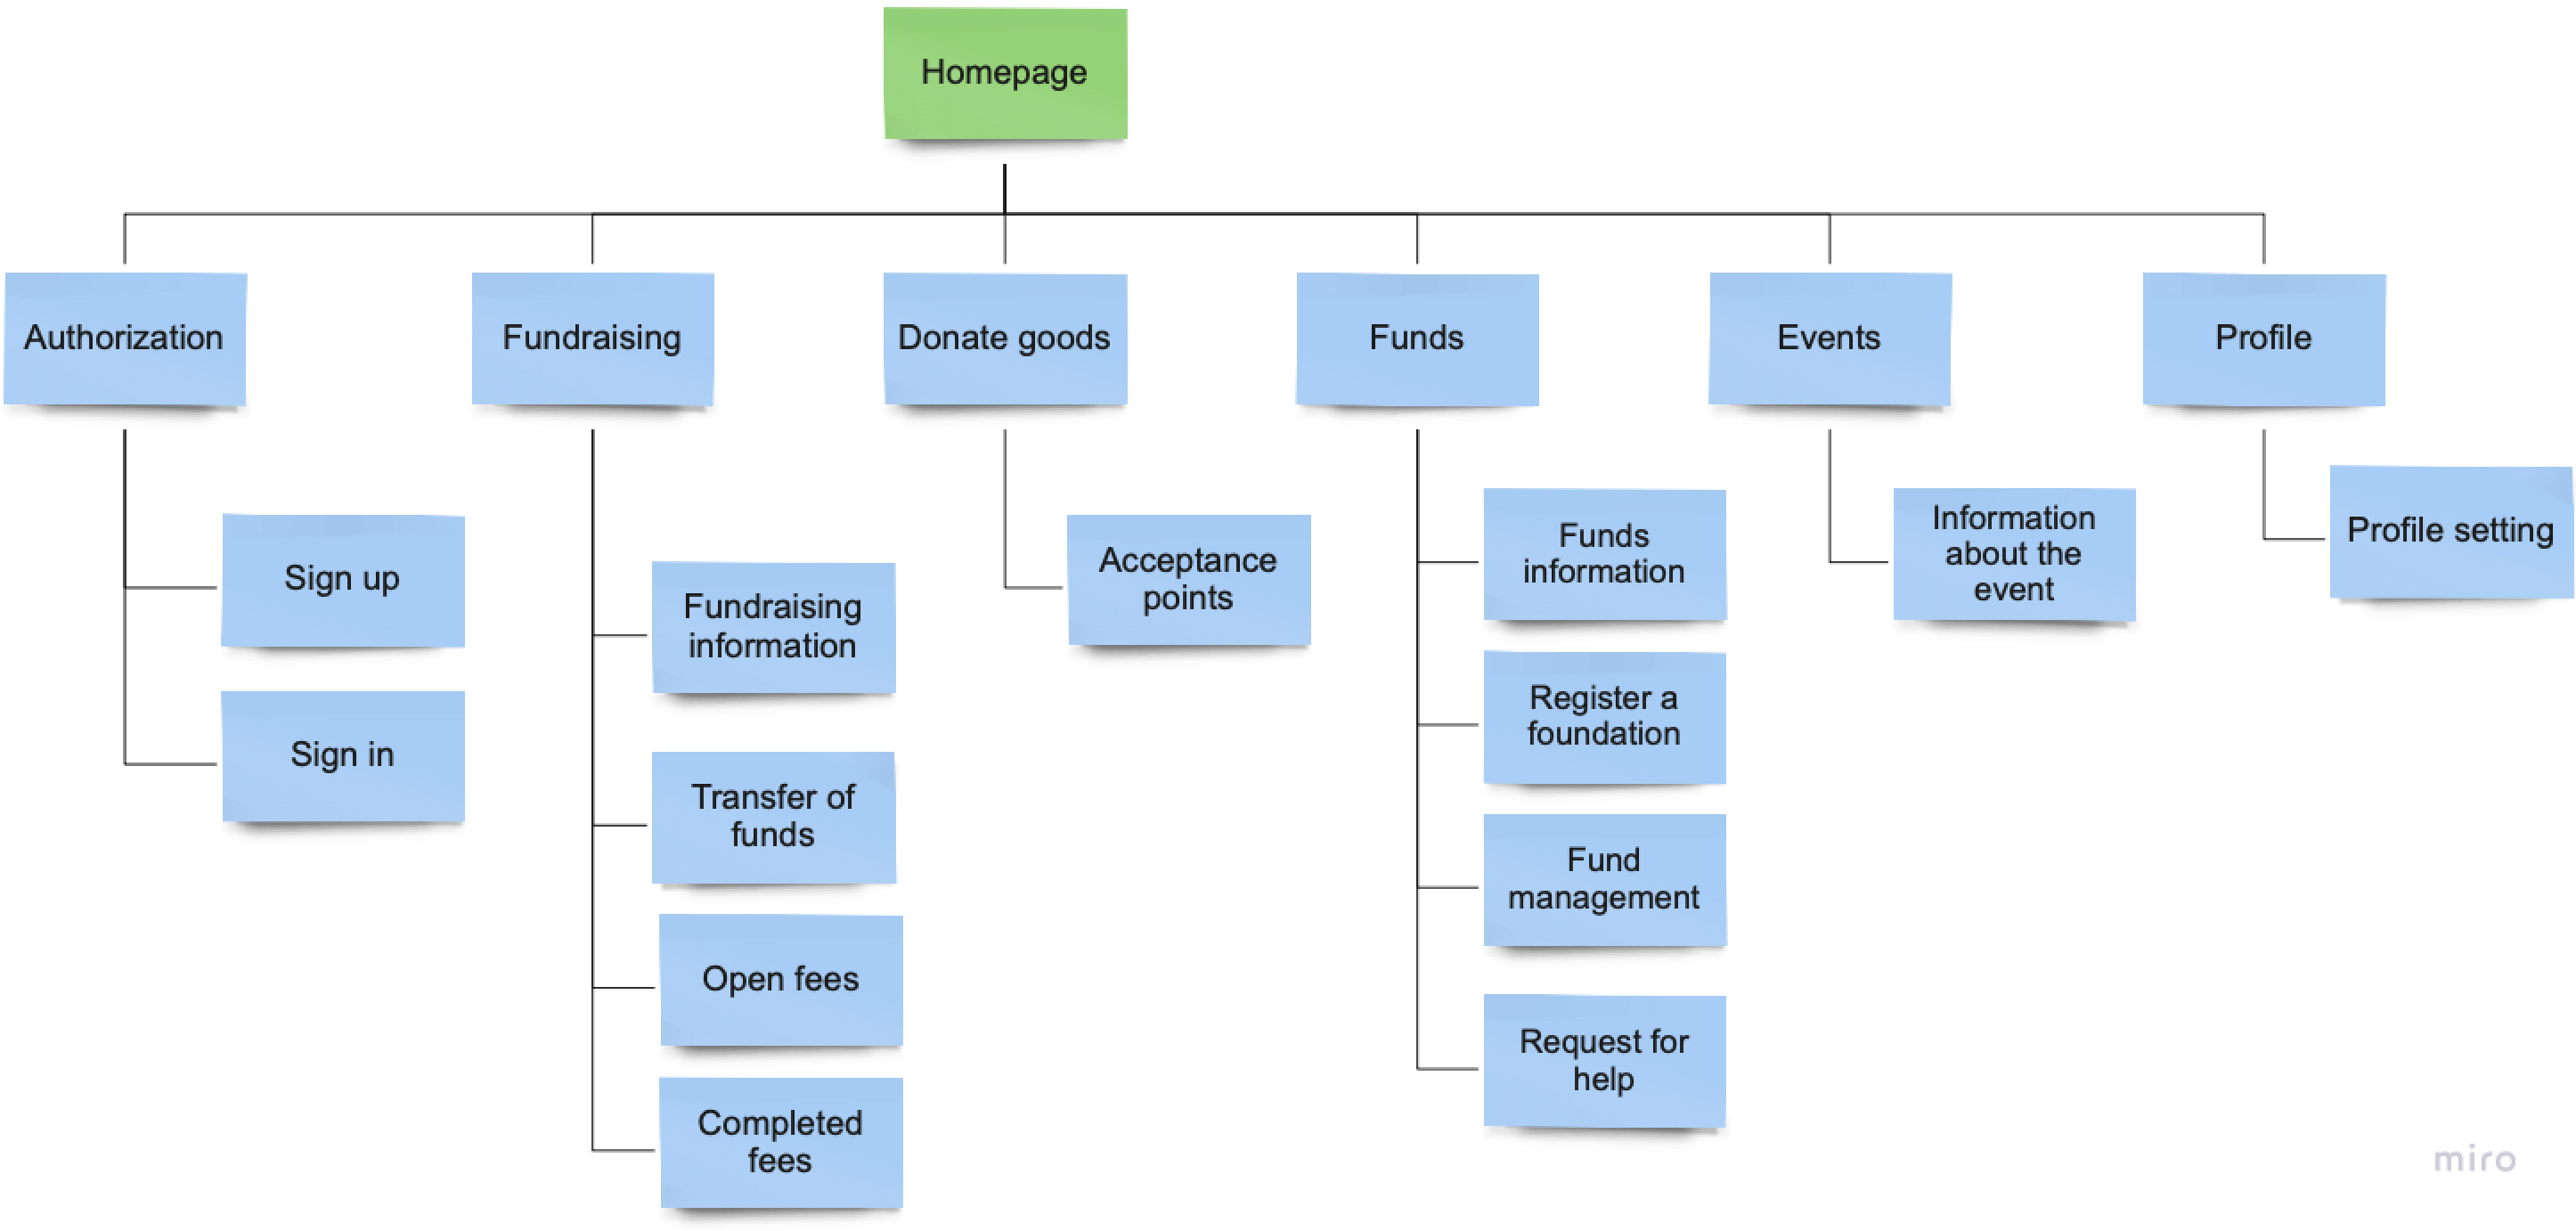
\includegraphics[width=12cm]{figures/userInterface/sitemap.jpg}
    \caption{Sitemap}
    \label{fig:sitemap}
\end{figure}

We used the \textbf{mind map} to build a connection between various elements of the application and
for a detailed description of the functionality of the elements

% mindmap
\begin{figure}[h]
    \centering
    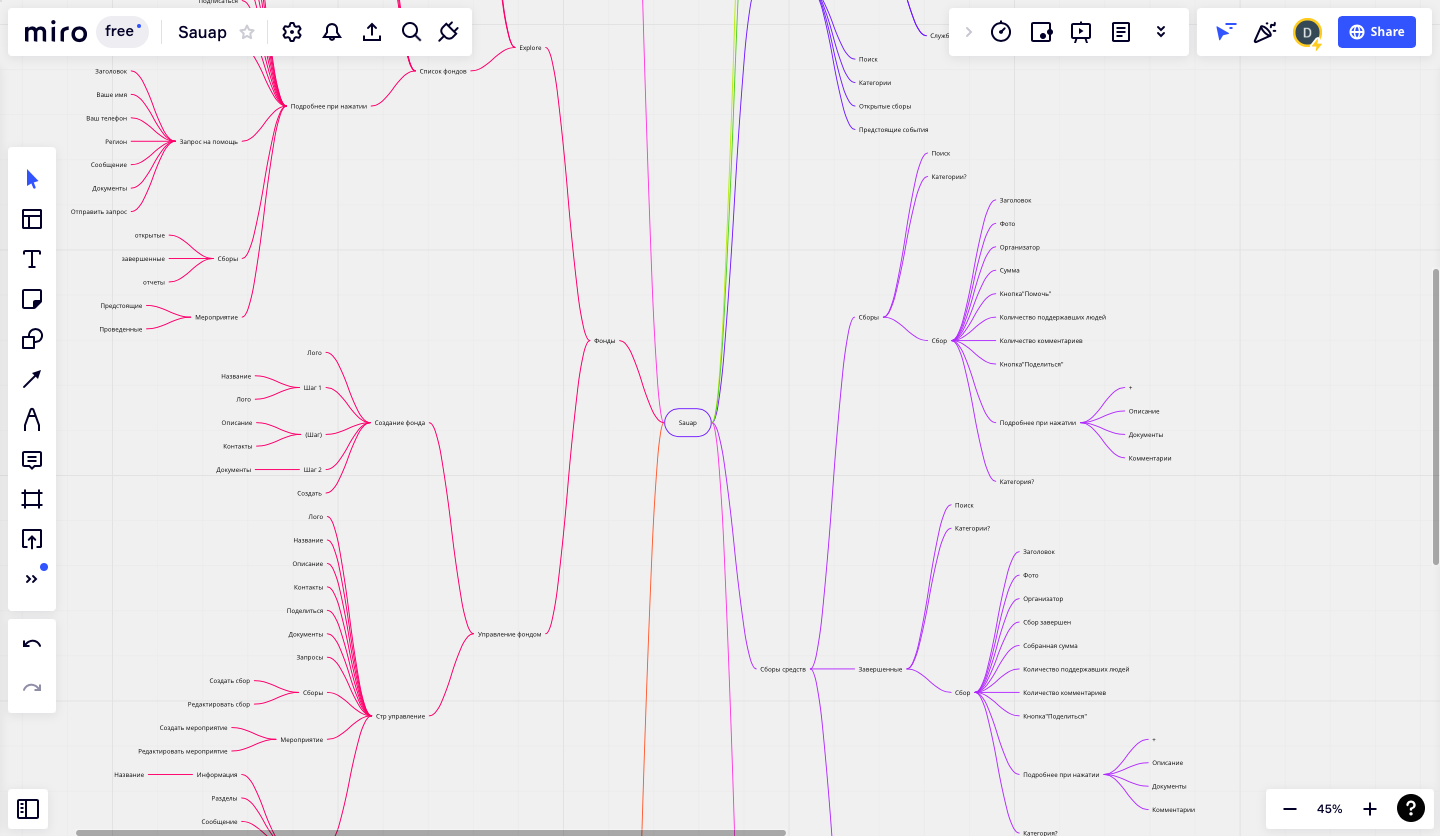
\includegraphics[width=12cm]{figures/userInterface/mindmap.png}
    \caption{Mind map}
    \label{fig:userFlow}
\end{figure}

All these methods helped us to form the User Experience, that is, to determine the needs,
wishes and behavior of the user. The data collected through these methods became the basis of
the next stage - prototyping.

\subsection{Wireframe}

Wireframe is the initial stage of creating an interface design that shows the main groups of
content, their location and general interface features.

We used Wireframe to show how the interface works without going into graphic design details.
This allowed the team to evaluate the basics of user interaction in the early stages.

First, to visualize our idea, we started to draw a prototype on paper (a low-level wireframes).

% wireframe 1 image
\begin{figure}[h]
    \centering
    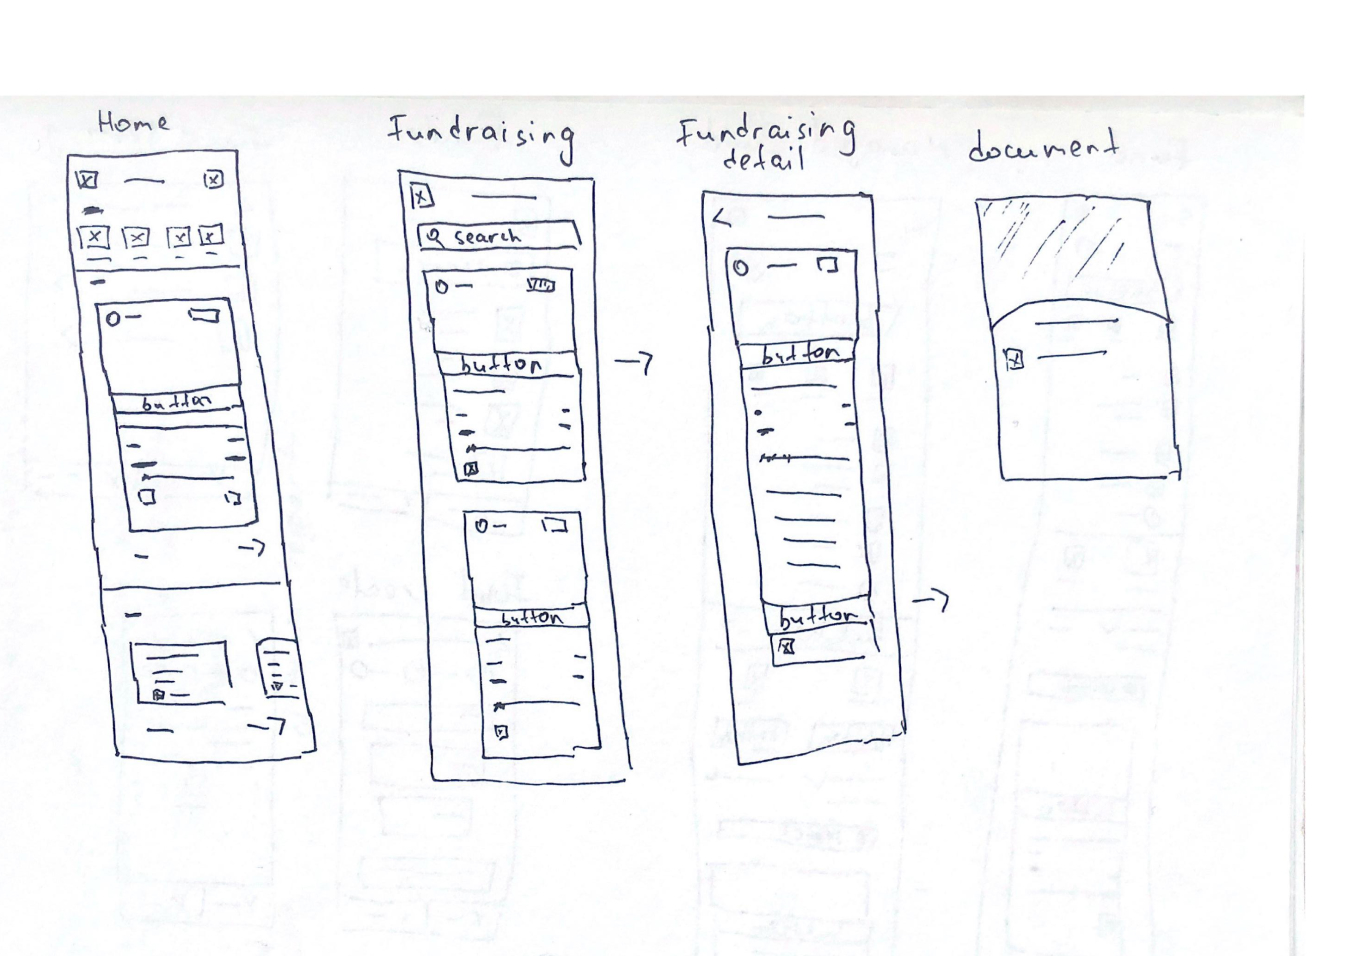
\includegraphics[width=10cm]{figures/userInterface/wireframe_low-fi_1.jpg}
    \caption{Wireframe low}
    \label{fig:wireframelow}
\end{figure}

Then we edited some elements and prototypes. Having approved the prototype structure with
the team, we began to draw high-level wireframes on the figma.

% wireframe 2 image
\begin{figure}[h]
    \centering
    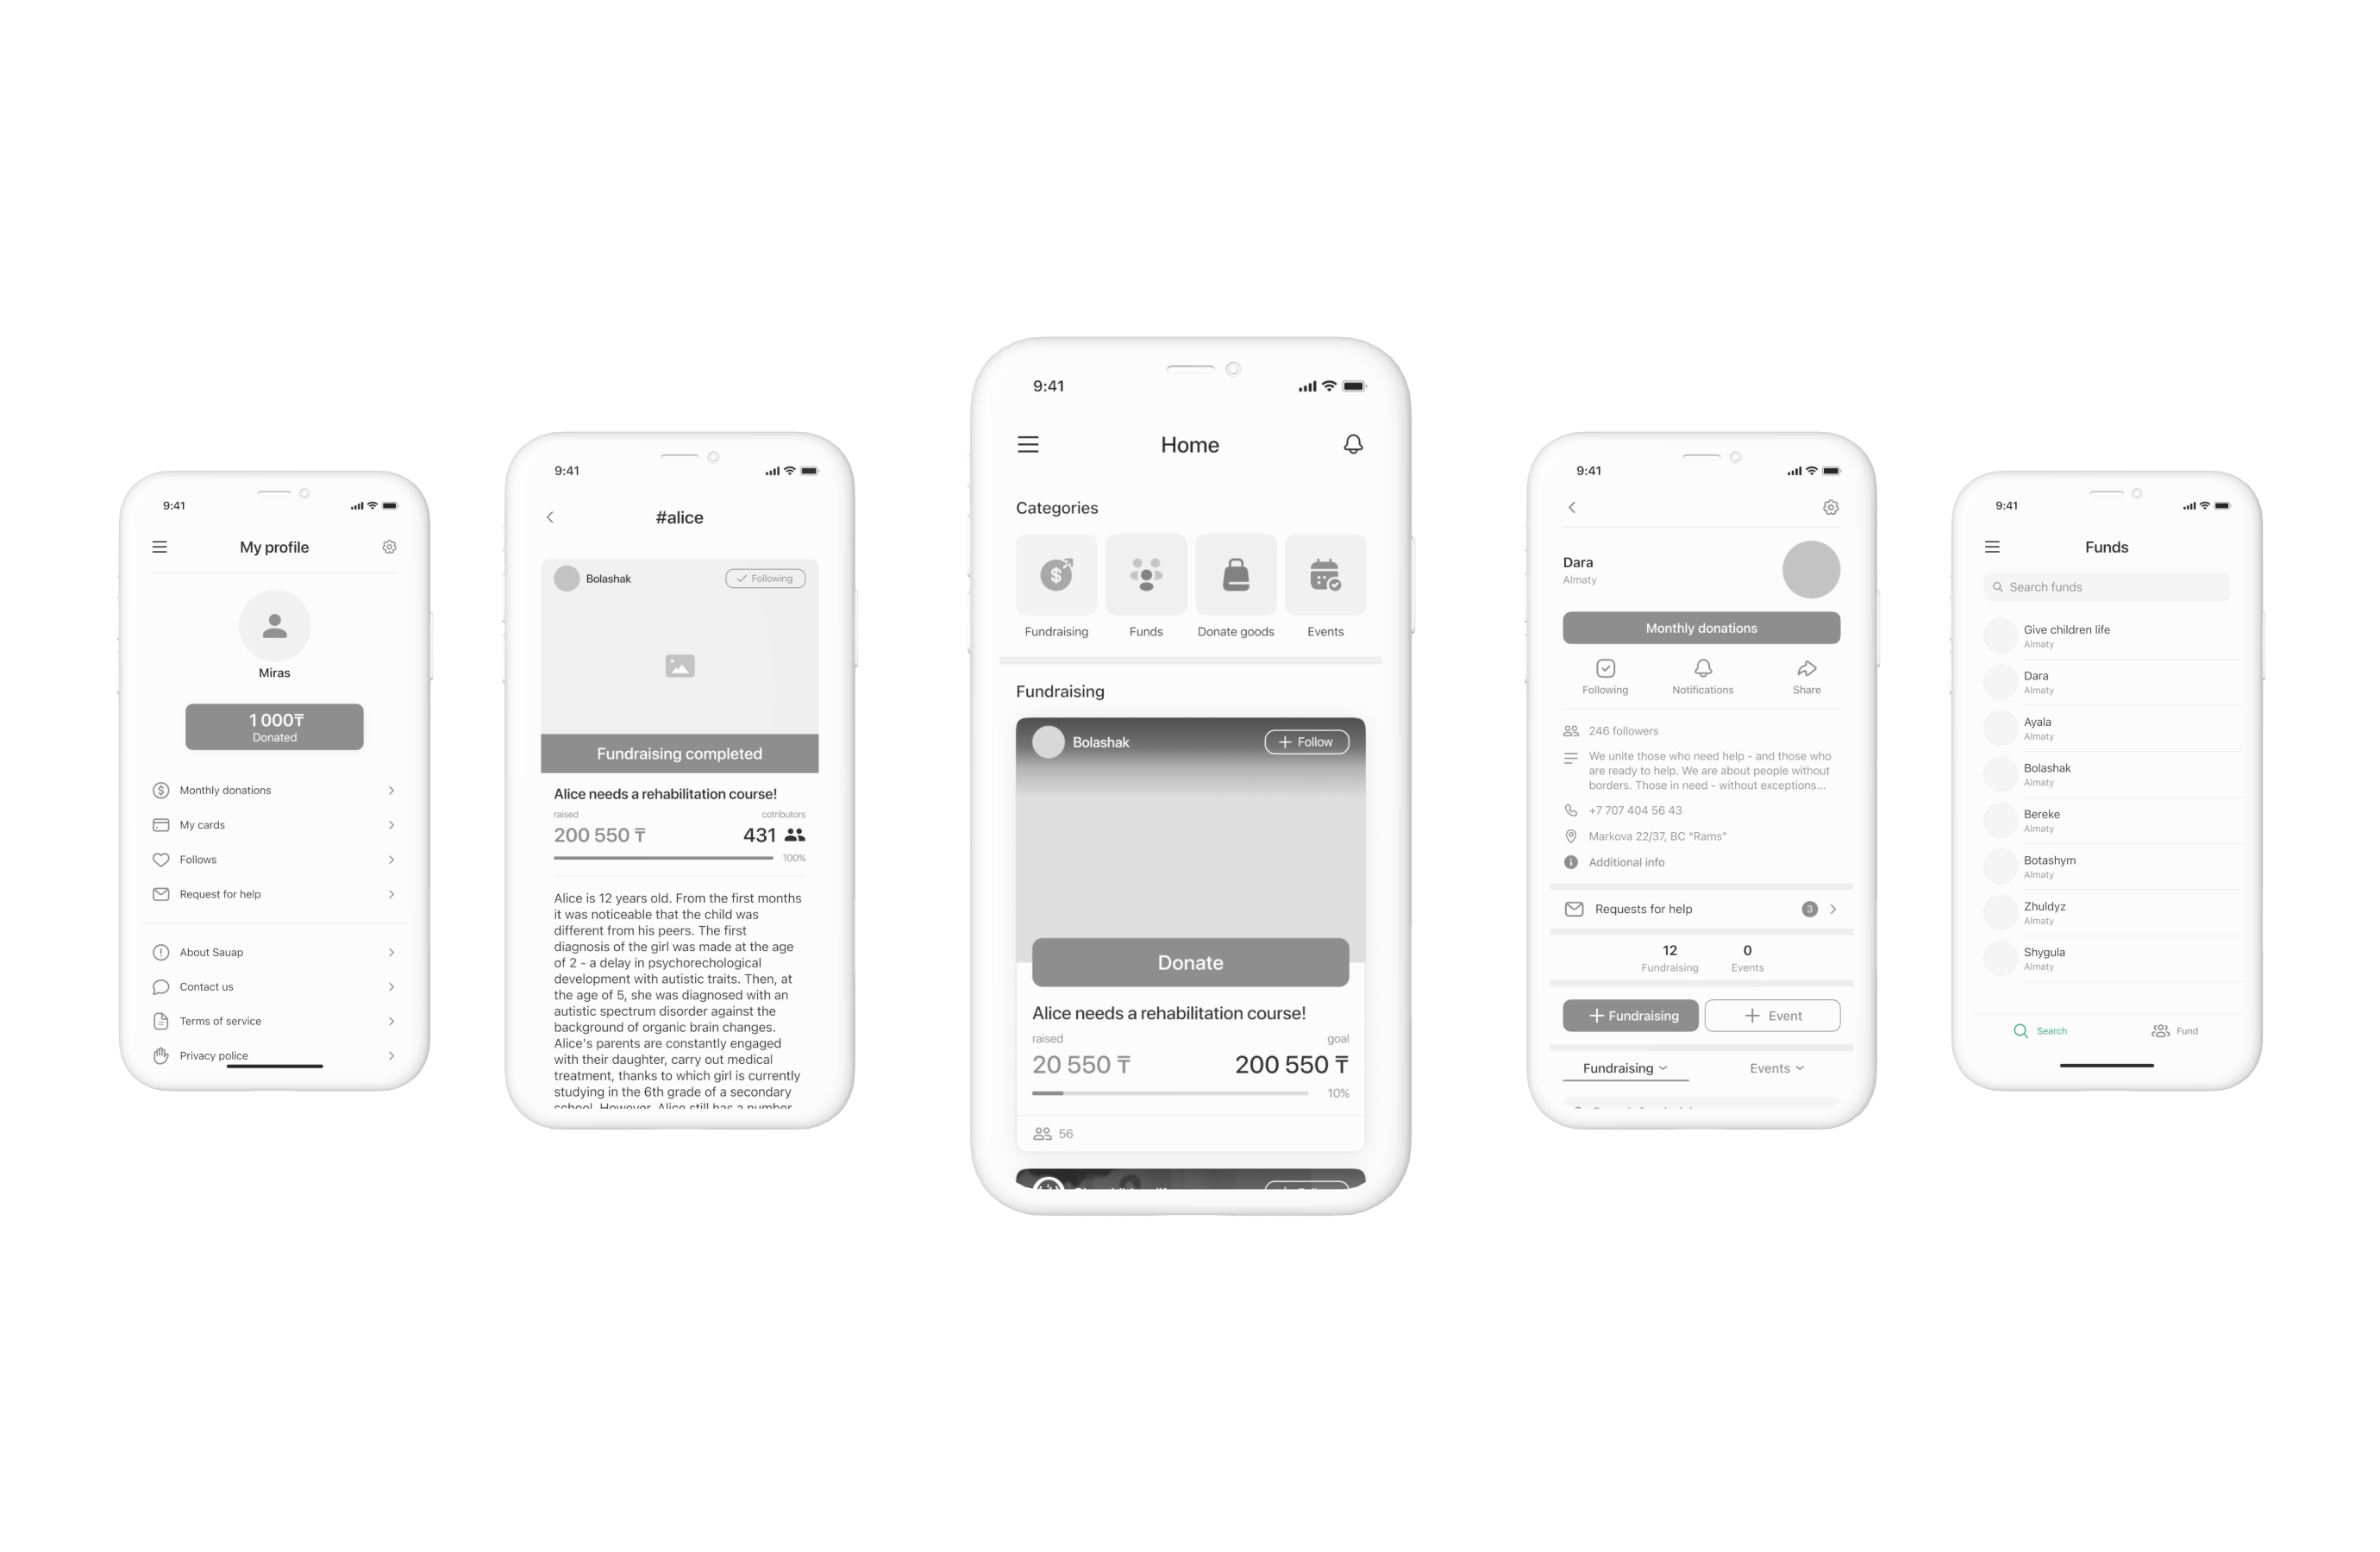
\includegraphics[width=10cm]{figures/userInterface/wireframe_hi-fi_1.jpg}
    \caption{Wireframe high}
    \label{fig:wireframehigh}
\end{figure}

\subsection{Visual design}

Our diploma project is dedicated to charity work and we carefully selected colors to
convey the meaning of our application. The main color of the application is green, according to the psychology of colors, green is considered the color of life, trust and lightness. As well as secondary colors such as: blue, purple, pink, orange. 

All design elements have rounded corners, which demonstrates a ‘friendly’ interface, as well as the buttons are easy to press, and there is enough space between the buttons for convenient clicking on them.

On the first page, the user can immediately make a donation in one click, or go to the page he needs.

\subsection{Mockup}

After the UI design part, we moved on to the next design stage, creating a clickable prototype on figma to visually see how the final product will work.

% mockup image
\begin{figure}[h]
    \centering
    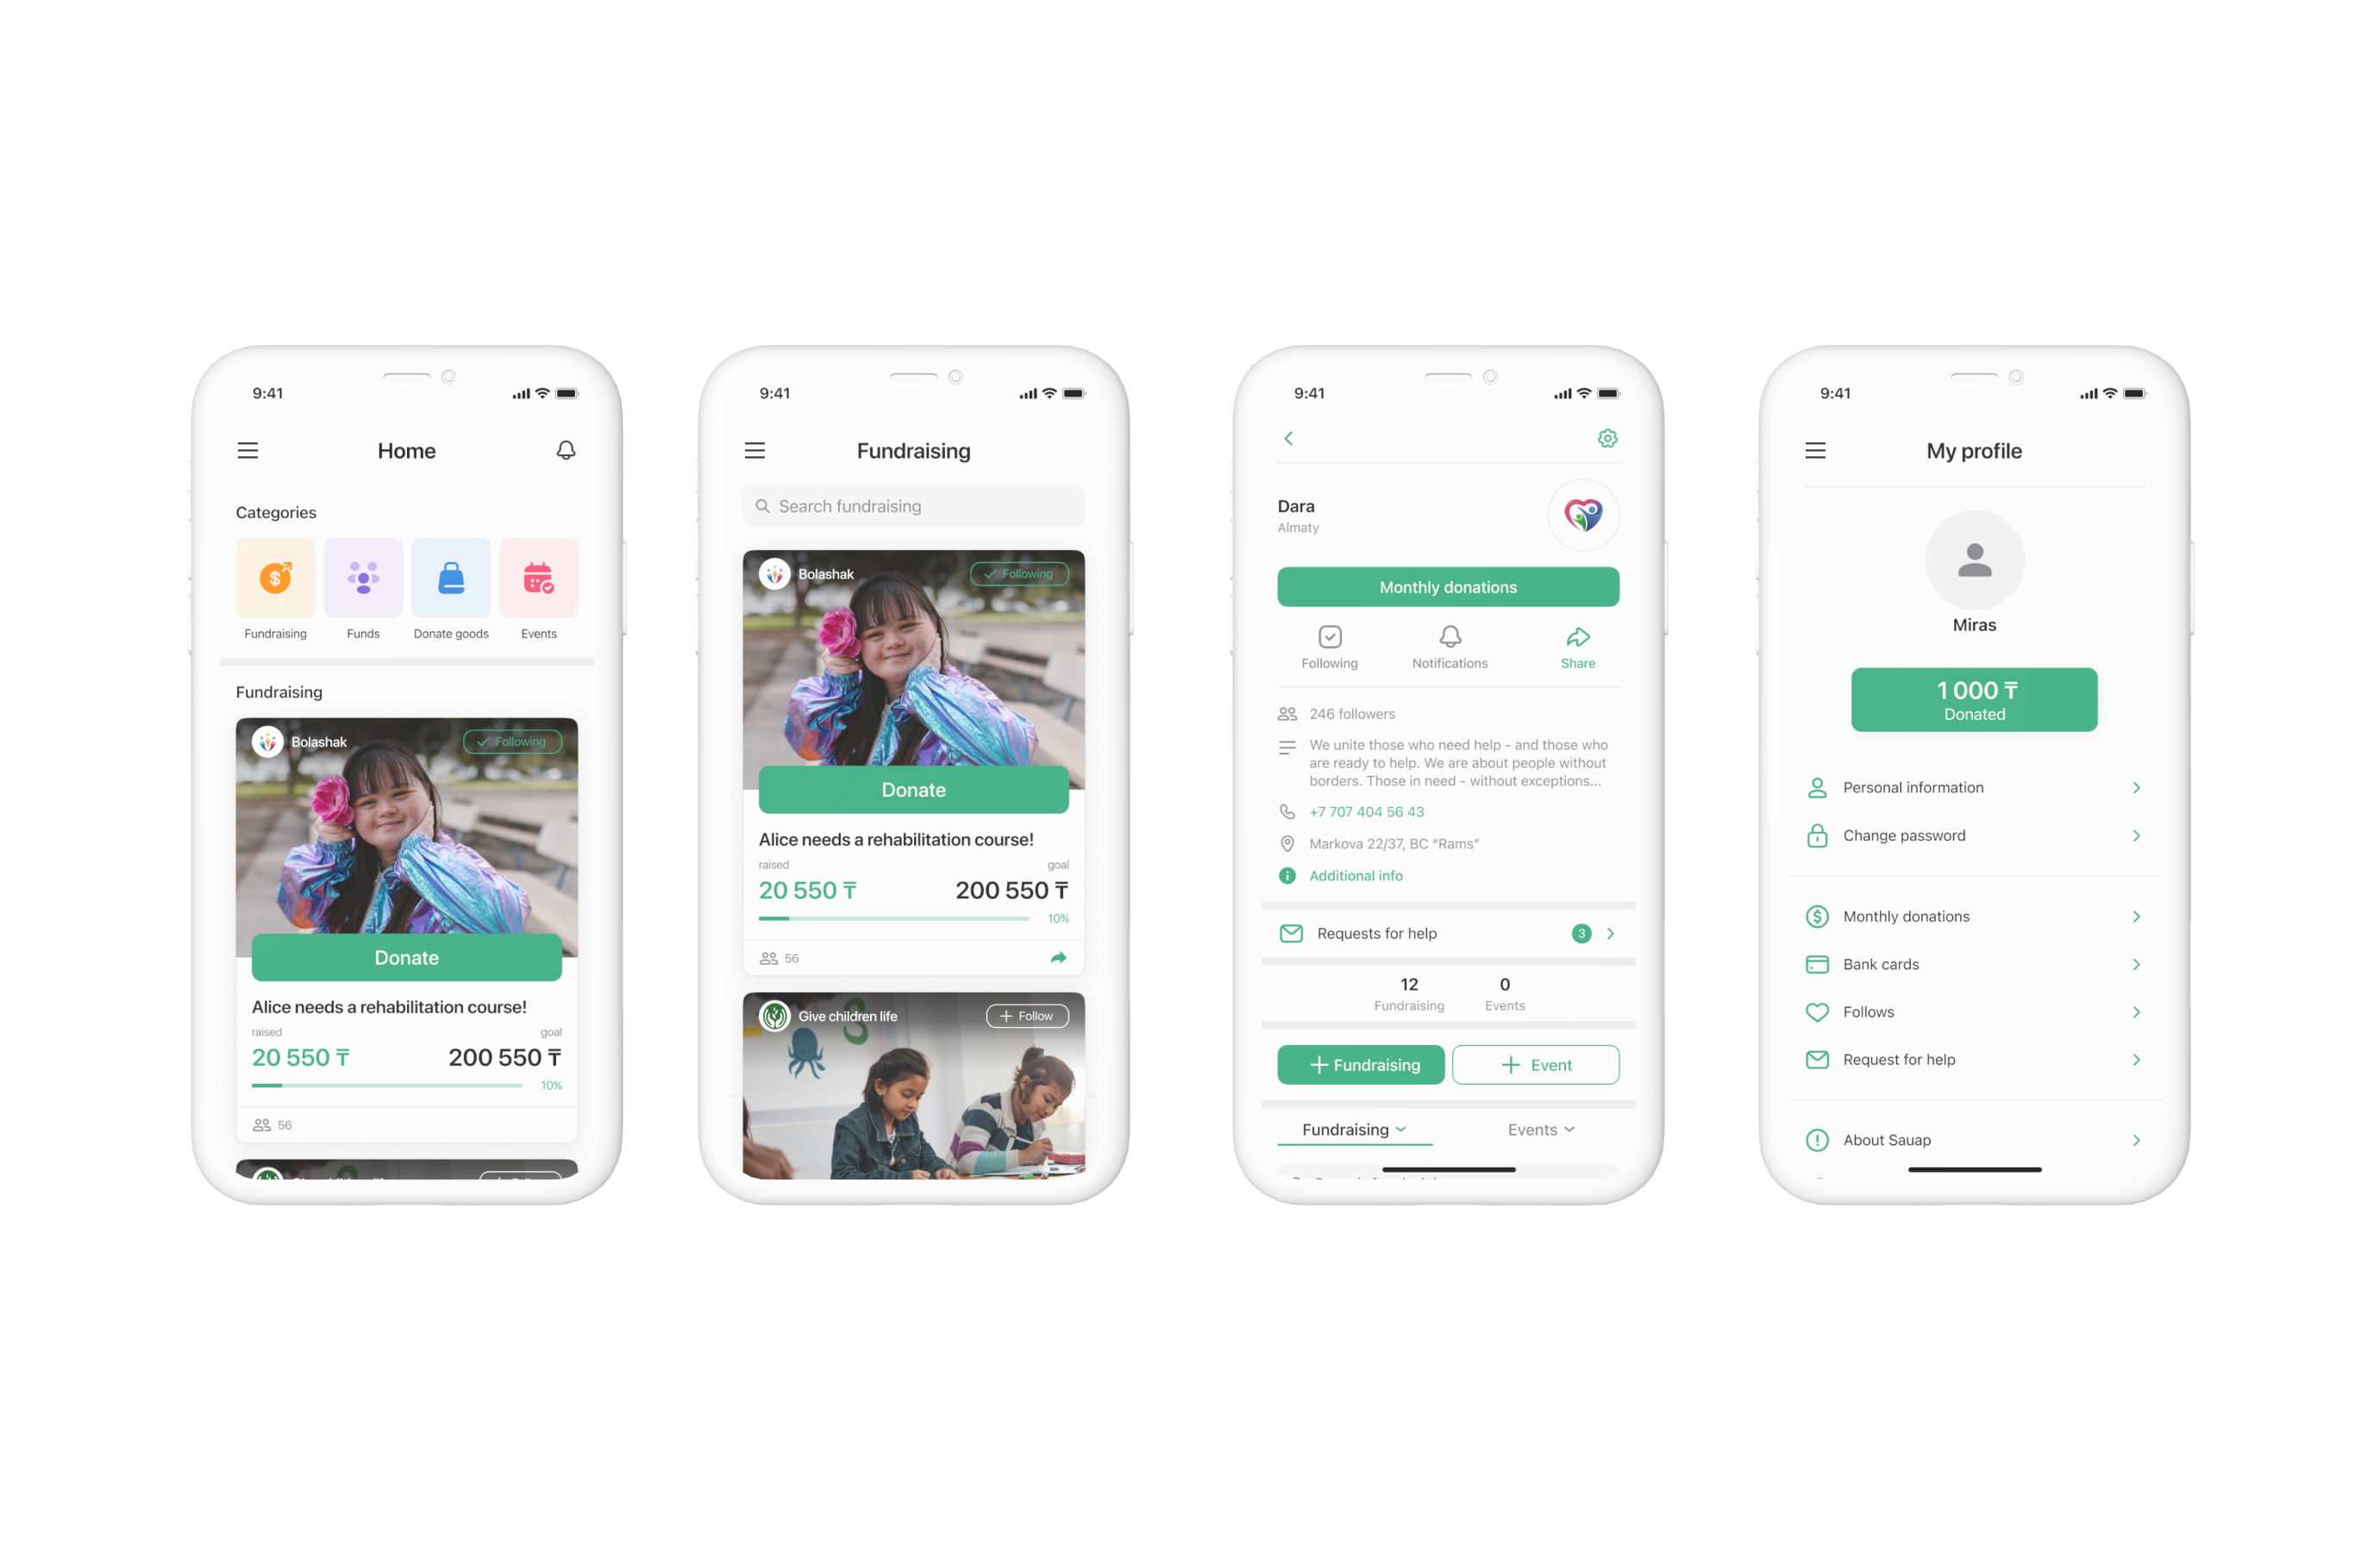
\includegraphics[width=11cm]{figures/userInterface/mockups.jpg}
    \caption{Mockup}
    \label{fig:mockup}
\end{figure}